\section{基准U-Net模型设计与实现}

\subsection{数据集准备与预处理}

\subsubsection{ISBI皮肤镜影像数据集}

ISBI皮肤镜影像数据集(2018年)由国际皮肤影像协作组织(International Skin Imaging Collaboration, ISIC)联合Memorial Sloan Kettering Cancer Center、University of Queensland等多家机构共同构建,并作为ISIC 2018皮肤病变识别挑战赛(ISIC Challenge 2018)的官方数据资源\cite{codella2019skinlesionanalysismelanoma}。该挑战共设立了三项任务:皮肤病变分类、像素级病变区域分割以及病变属性预测,数据集也据此提供了相应的图像与标注文件。

ISIC 2018数据集作为目前最具影响力的皮肤镜数据集之一,广泛用于皮肤病变分割与分类模型的基准测试。数据集总共包含2594张RGB三通道皮肤镜图像,图像格式为JPEG或PNG,分辨率在600×450至6748×4499像素之间,保留了丰富的病变细节特征(如色素网、结构不规则性、色斑边缘模糊等),图像采集过程遵循标准化的成像协议(如偏振光皮肤镜)。除图像本体外,每张图像还附带包括患者年龄、性别、病变解剖部位等在内的临床元数据,具备一定的多模态分析潜力。

在标注方面,数据集提供由皮肤科专家精确勾画的像素级病变掩膜用于病变区域分割任务训练,掩膜的标注一致性通过交叉验证确认(Kappa 系数大于 0.82)。同时,整个数据集按照任务需求被官方划分为训练集(2,000 张,含掩膜和标签)、验证集(300 张,仅标签)与测试集(294 张,无公开标注,仅用于模型评估)。

为确保输入数据的一致性与模型训练的稳定性,本研究对ISIC 2018皮肤镜影像数据集中的图像及其对应的掩膜进行了标准化预处理。所有RGB皮肤镜图像统一归一化至$(0,1)$范围,掩膜转换为双通道概率标签(0-背景,1-病变),为后续使用基于概率分布的损失函数(如交叉熵损失、Dice损失)提供结构支持。

为确保训练过程的可控性与评估结果的可靠性,数据集严格遵循官方划分比例(训练集:验证集:测试集=70\%:15\%:15\%),通过随机分层抽样确保分布一致性,避免评估偏差。

\subsubsection{LiTS肝脏CT数据集}

LiTS(Liver Tumor Segmentation)数据集是由MICCAI 2017肝脏肿瘤分割挑战赛(Liver Tumor Segmentation Challenge 2017)发布的医学影像公开数据集,由来自全球多家权威医疗机构提供的腹部增强CT扫描组成,涵盖130例临床病例,包含多种肝脏病理状态,包括肝细胞癌、转移性肿瘤、胆管细胞癌等\cite{Bilic_2023}。所有图像数据均采用静脉期CT成像,层厚范围为1–5mm,横断面矩阵分辨率为512×512,体素间距在0.6–1.0 mm之间(存在一定程度的各向异性)。成像窗宽窗位统一设定为肝脏窗(窗宽150–200 HU,窗位约-50–50 HU),以增强肝实质与病灶之间的密度对比。

在标注方面,数据集中每一病例均由三位经验丰富的放射科专家进行独立标注,提供像素级肝脏与肿瘤分割掩膜。标注一致性通过Dice系数(平均大于0.92)和Hausdorff距离(平均小于5 mm)进行验证,部分病例还附带有病灶的病理学分型标签。

LiTS 2017数据集的挑战性体现在多方面:其一,肝脏轮廓复杂、变异性大,且边界常与胃肠道等邻近脏器重叠,导致区域判别困难;其二,肿瘤病灶形态异质性强(如结节型、融合型、浸润型),并存在大小悬殊、边界模糊、低密度病灶等不利因素;此外,呼吸运动伪影与层间不连续性也显著增加了分割任务的难度。

在模型训练前,本研究对LITS 2017肝脏CT数据集进行了系统性预处理,以确保数据一致性与模型输入的可靠性。所有CT图像以伪彩色映射形式统一读取为RGB三通道格式,并转换为浮点张量,数值范围归一化至$(0,1)$;对应的单通道掩膜(0表示背景,1表示肝脏及肿瘤区域)同步转换为张量格式,针对二分类任务需求,掩膜进一步编码为双通道概率标签(通道0为背景概率,通道1为前景概率),以适配基于概率分布的损失函数。数据集严格遵循预定义划分策略,通过固定随机种子生成可复现的训练集、验证集与测试集分配方案。此外,文件名经匿名化处理,患者隐私信息完全脱敏,符合医学伦理规范。整体流程通过标准化映射、严格划分与一致性校验,为肝脏肿瘤分割任务构建了高鲁棒性的数据基础。

\subsubsection{BraTS脑肿瘤MRI数据集}

BraTS(Brain Tumor Segmentation)2020 数据集由 MICCAI 组织联合宾夕法尼亚大学、慕尼黑工业大学等多家国际顶尖医学与工程研究机构共同构建,作为年度脑肿瘤分割挑战赛的重要基准数据资源\cite{menze2015}。该数据集专注于胶质瘤(包括高级别胶质瘤HGG与低级别胶质瘤LGG)MRI图像的分割任务,广泛用于评估多模态影像分割算法的性能与鲁棒性。

数据集中共包含 369例患者的多模态MRI扫描数据,每例数据均包含四种标准MRI模态:T1加权(T1)、T1对比增强(T1ce)、T2加权(T2)以及液体衰减反转恢复序列(FLAIR)。所有图像均经过统一预处理流程,包括:

\begin{enumerate}
    \item 各向同性重采样至1.0×1.0×1.0 mm³体素分辨率
    \item N4偏场校正以消除非均匀磁场引起的信号漂移
    \item 跨模态配准,确保不同模态间空间对齐一致。
\end{enumerate}

在数据标注方面,每例数据均提供由神经放射学专家联合标注的像素级三维分割掩膜,标注内容涵盖:

\begin{enumerate}
    \item 增强肿瘤区域(Enhancing Tumor,ET):表现为对比增强T1序列中具有强化表现的病灶区域;
    \item 肿瘤核心(Tumor Core,TC):包括坏死区域、实性肿瘤与增强部分;
    \item 肿瘤整体(Whole Tumor,WT):包括肿瘤核心与周围水肿区域。
\end{enumerate}

BraTS 2020数据集的主要挑战包括:(1)肿瘤组织的高度异质性,如增强区与坏死区边界模糊;(2)小体积或卫星灶的检测难度高,极易被误判或遗漏;(3)多模态之间的病灶表征差异显著,对模型特征融合能力提出更高要求。

为构建高效且可复现的脑肿瘤分割数据管线,本研究基于BraTS 2020数据集设计了系统化预处理流程。首先,所有病例按目录名排序并剔除损坏样本,采用两级随机划分策略:10\%病例作为独立测试集,剩余病例在固定随机种子控制下进一步分为训练集(70\%)与验证集(20\%),病例ID分配方案持久化为JSON文件以确保实验可复现性并避免数据泄漏。

不同于ISBI 2018和LiTS 2017数据集,针对BraTS数据集是多模态数据的情况,仅采用FLAIR和T1对比增强两种模态组合作为输入序列,有研究表明对于脑肿瘤语义分割任务,这种序列组合是最佳的组合选择\cite{buchner2023}。此外,所有输入数据逐例归一化至$(0,1)$范围以消除扫描设备差异,并遍历三维体积数据的轴向切片,剔除无标注信息的空白切片(分割掩膜全零),缓解类别极端不平衡问题;对原始标签(增强肿瘤、肿瘤核心、坏死区)按临床需求重映射为统一类别体系,并转换为多通道one-hot编码,适配交叉熵损失与Dice损失的监督需求。

总结来说,每张切片被组织为2-通道输入(FLAIR + T1ce)和4通道one-hot标签,按批次送入数据流水线。管线支持随机打乱、动态批量组装、并行预取和可选重复迭代,从而在保证 I/O 吞吐的同时充分混洗样本。

\subsection{基准U-Net模型构建}
%详细描述U - Net模型的构建过程,包括网络层的搭建、损失函数的选择(如Dice损失函数)等。
%训练过程中的参数设置,如学习率、批量大小、训练轮数等。
本研究在经典U-Net框架的基础上实现了基准U-Net模型的构建,用以评估后续改进策略的真实收益。模型构建包括网络层的搭建、损失函数的涉及和优化器的选择。

\subsubsection{网络层}

图~\ref{fig:unet_ushape}展示了本研究搭建的基准U-Net模型的模型架构,网络采用对称的编码器—解码器结构:

编码端连续堆叠四级特征抽取单元,每一级由两层3×3有填充卷积与ReLU激活组成;特征通道数以32为起始,在每次下采样后按1∶2的比例递增(即32→64→128→256)。空间下采样通过2×2最大池化实现,使特征图尺寸依次减半,从而在更大的感受野上编码语义信息。

解码端采用与编码端对称的结构,对最深层特征进行转置卷积上采样,并与对应级别的编码器输出进行特征级串接后,执行两层卷积+激活以还原局部细节。此跳跃连接在保持全局上下文同时弥补高分辨率细节缺失,是U-Net能够兼顾定位精度与类别判别力的关键机制。最终输出层采用1×1卷积,将通道数映射为$C$($C$为分割图的像素类别数),输出未经激活直接送入损失函数计算,以便在训练阶段灵活选择Sigmoid或Softmax型损失。

\begin{figure}
    \centering
    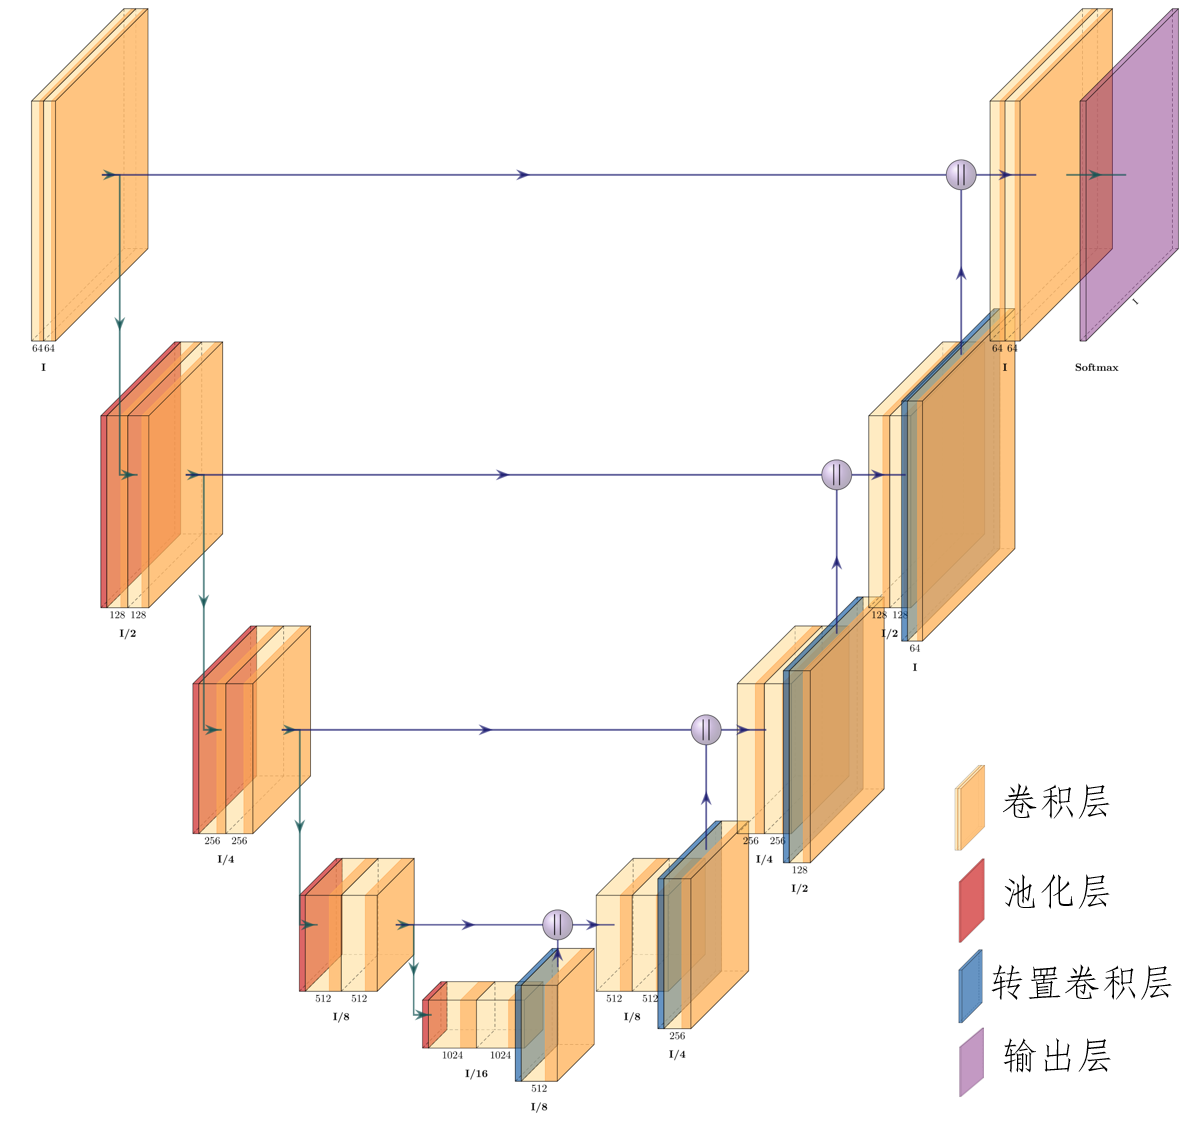
\includegraphics[width=\textwidth]{fig/Unet_ushape.png}
    \caption{fig:unet_ushape}
    \label{fig:unet_ushape}
\end{figure}

上述网络拓扑及通道配置均采用Pytorch框架实现,对应的实现要点可在附录A中进一步查证。

\subsubsection{损失函数的设计}

在损失函数的设计上,本文采用Dice – Cross-Entropy混合损失(以下简称混合损失),即以相等权重线性叠加Dice损失与像素级交叉熵(CE)损失,以充分兼顾类别不平衡下的区域重叠度优化与梯度稳定性。设网络输出的类别概率图(像素总数为$N$)为:$ P=\left\{p_{i}\right\}_{i=1}^{N} $,真实分割掩膜为$ G=\left\{g_{i}\right\}_{i=1}^{N} $,其中$ p_{i} \in[0,1], g_{i} \in\{0,1\}$分别是像素$i$的前景概率和真实标签。则:

\begin{equation}
    \mathcal{L}_{\text {Dice }}=1-\frac{2 \sum_{i=1}^{N} p_{i} g_{i}}{\sum_{i=1}^{N} p_{i}+\sum_{i=1}^{N} g_{i}+\varepsilon}
\end{equation}

\begin{equation}
    \mathcal{L}_{\mathrm{CE}}=-\frac{1}{N} \sum_{i=1}^{N}\left[g_{i} \ln \left(p_{i}\right)+\left(1-g_{i}\right) \ln \left(1-p_{i}\right)\right]
\end{equation}

\begin{equation}
    \mathcal{L}_{\text {mix }}=0.5 \mathcal{L}_{\text {Dice }}+0.5 \mathcal{L}_{\mathrm{CE}}
\end{equation}

其中$ \varepsilon=10^{-6} $用于数值平滑以防零分母。Dice项直接对预测与标注的重叠区域进行归一化度量,能在小体积病灶场景下显著提升召回;交叉熵项则提供像素级对数似然的密集监督,改善早期训练阶段梯度稀疏、收敛震荡等问题。

\subsubsection{优化器的选择}

优化器采用Adam随机梯度下降算法,其一阶自适应动量可在早期快速探索有效学习率区间,同时在震荡平衡阶段保持较小更新幅度。初始学习率设定为$ 1.0 \times 10^{-4} $,一阶、二阶动量系数沿用默认值$ \beta_{1}=0.9, \beta_{2}=0.999 $。

\subsection{训练策略与评估指标}

\subsubsection{训练策略}

模型的训练均在Kaggle平台进行,采用Kaggle平台提供的NVIDIA P100 (16 GB) 单卡进行模型加速训练。

为了避免训练后期进入平台期,附加 Reduce-on-Plateau 学习率调度策略:当验证集指标在 10 个 epoch 内无显著提升时,将学习率衰减为原值的 0.5;最低学习率限定在$ 1.0 \times 10^{-6} $,防止数值下溢而不再更新参数。当学习率因多次衰减而触碰下限时,若模型仍无改善,则提前终止训练以节省算力。

训练超参数经预实验网格搜索确定:批量大小根据数据集的规模和大小确定,完整训练周期设置为100epoch,保证验证过程与训练同步,本研究在每个 epoch 结束后立即于验证集评估 Dice 系数并记录最优权重;测试集仅使用单尺度推断,不采用多尺度或模型集成,确保基准模型公平、简洁、可复现。

\subsubsection{评估指标}

在医学图像分割研究中,模型输出通常为与输入图像同尺寸的二值概率图,衡量其与专家标注掩膜之间的相似程度是评价算法优劣的关键。单一指标无法满足同时反映检测率、误诊率和重叠精度的要求,多指标可立体呈现模型表现。因此,在本研究中,我们以混淆矩阵四要素——真阳性(TP)、真阴性(TN)、假阳性(FP)、假阴性(FN)——为基础,记录Accuracy、Precision、Recall、Specificity、F1-Score、Dice系数与Jaccard指数七项指标。下面逐一给出指标定义、公式及其评价意义。

准确率Accuracy表示正确预测的样本占总样本的比例,是最直观的分类性能指标:

\begin{equation}
    \mathrm{Accuracy}=\frac{TP+TN}{TP+TN+FP+FN}
\end{equation}

Accuracy直观反映模型的综合判断能力,但在病灶面积远小于背景时,Accuracy易受TN主导,可能高估模型质量,因此仅作为参考基线。

精确率Precision表示预测为正类的样本中实际为正类的比例,反映模型的预测可靠性:

\begin{equation}
    \mathrm{Precision}=\frac{T P}{T P+F P}
\end{equation}

Precision反映模型整体预测正确性,但在类别极度不平衡时(如背景像素占比90\%以上),可能高估性能(例如模型仅预测背景即可获得高准确率),需结合其他指标综合判断。

F1-Score是精确率(Precision)与召回率(Recall)的调和平均数,综合衡量模型在正类样本上的分类能力,尤其适用于类别不平衡场景:

\begin{equation}
    \mathrm{F} 1=\frac{2 T P}{2 T P+F P+F N}=2 \cdot \frac{\text { Precision } \times \text { Recall }}{\text { Precision }+ \text { Recall }}
\end{equation}

F1分数可以避免仅关注单一指标(如高精确率但低召回率),在医学图像分割中(如肿瘤区域占比小),能更均衡评估模型对正类(病变区域)的捕捉能力与预测准确性。

Dice系数衡量预测结果与真实标签的重叠程度,是医学图像分割的核心评估指标:

\begin{equation}
    \mathrm{Dice}=\frac{2 T P}{2 T P+F P+F N}=\frac{2 \times|A \cap B|}{|A|+|B|}
\end{equation}

其中,A为预测区域,B为真实区域。Dice系数直接衡量空间重叠,对不平衡数据敏感度低,能有效评估模型对病灶轮廓的捕捉精度,尤其适用于小目标分割任务(如脑肿瘤核心)。

召回率Recall召回率表示实际为正类的样本中被正确预测的比例,反映模型对正类样本的覆盖能力:

\begin{equation}
   \mathrm{Recall}=\frac{T P}{T P+F N} 
\end{equation}

高召回率意味着模型能有效捕捉病变区域(减少漏检),在早期诊断(如癌症筛查)中至关重要,但需平衡精确率以避免过度预测。

特异性Specificity表示实际为负类的样本中被正确预测的比例,衡量模型识别阴性样本的能力:

\begin{equation}
    \mathrm{Specificity}=\frac{T N}{T N+F P}
\end{equation}

在医学任务中,高特异性可减少健康组织被误判为病变的风险(如避免正常脑组织被误分割为肿瘤),提升结果的可信度,与 Recall 形成互补。

Jaccard指数(IoU)计算预测与真实标签的交集与并集的比值,是分割任务的经典指标:

\begin{equation}
    \mathrm{Jaccard}=\frac{T P}{T P+F P+F N}=\frac{|A \cap B|}{|A \cup B|}
\end{equation}

其中,A为预测区域,B为真实区域。Jaccard指数严格量化重叠区域的比例,对分割边界的轻微偏移敏感,常用于评估模型在复杂解剖结构(如肿瘤浸润区域)中的细节保留能力,在多模型比较时可提供更保守的评估视角。